\chapter{Zastosowania w biznesie}
\label{ch:biznes}
 Technologia wirtualnej rzeczywistości zajmuje umysł rozmyślaniem nad nieskończonymi możliwościami inwestorom, podmiotom biznesowym oraz twórcom od  dawna. Pomimo swoich początków w branży rozrywkowej coraz więcej osób dostrzega potencjał tej technologii w zastosowaniu biznesowym. Znajomość technologiczna pracowników pozwala na wdrożenie rozwiązań VR bez większych problemów a przypadki biznesowe dla których zostają wprowadzone rozwiązania z tej dziedziny często pozwalają na redukcje kosztów oraz czasu, w szczególności jeżeli porównywane jest to do odtworzenia danego środowiska w przestrzeni rzeczywistej, o ile to jest w ogóle możliwe. W wielu dziedzinach takich jak medycyna, motoryzacja, architektura czy lotnictwo coraz częściej liderzy decydują się na inwestycje oraz współpracę z firmami z obszarów XR, a dzięki przetartym szlakom, także kolejne branże coraz chętniej przyglądają się możliwościom zastosowania narzędzi pozwalających na tworzenie środowisk wirtualnych. Prognozy rynku przez takie firmy i agencje jak \textit{The Farm 51}, \textit{Tractica}, \textit{CCS Insight} czy \textit{SuperData} pokazują że wartość aplikacji oraz akcesoriów związanych z sektorem VR będzie ciągle rosnąć i stawać się coraz bardziej powszechna wśród użytkowników domowych, co sprawia że potencjał inwestycji dla wielu firm również wzrośnie, nawet jeżeli nie zdecydowały się one na wdrożenie rozwiązań technologicznych na chwilę obecną~\cite{raportVR}. Dzięki prężnemu rozwojowi technologii oraz coraz większemu zaufaniu tej technologii, miało szansę powstać wiele firm które nie tylko zajmuje się produkcją fizycznych komponentów o których wspomniano w rozdziale~\ref{ch:prezentacja}, ale także firmy które zajęły się wytwarzaniem oprogramowania oraz współpracy z klientami.
 \begin{figure}[h]
\centering
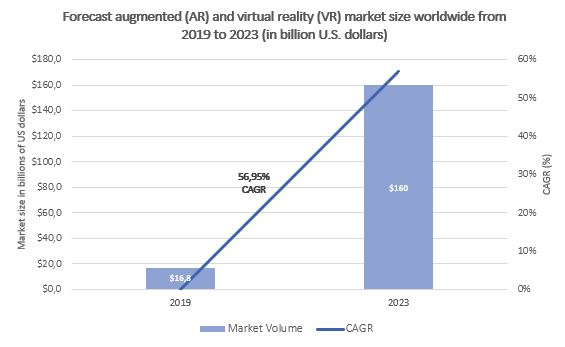
\includegraphics[width=\textwidth]{market}
\captionsource{Przewidywania wartości rynku AR i VR pomiędzy 2019 a 2023 rokiem}{\url{https://blog.camelot-group.com/2020/01/ar-vr-mr-science-fiction-or-science-fact/}}
\label{fig:market}
\end{figure}
  Firmy te zajmują się wytwarzaniem oprogramowania z którego mogą korzystać inne osoby w celu budowania własnych rozwiązań, firmy współpracujące z klientami i zajmujące się wdrażaniem ich pomysłów w życie, co często można zaobserwować w segmencie rozrywkowym a także jednostki zajmujące się produkcją oprogramowania z wyszczególnieniem danych sekcji przemysłowych, do których potrzebna jest bardziej szczegółowa wiedza i zazwyczaj firmy takie zajmują się tylko jednym rodzajem dostarczanych rozwiązań takich jak usprawnianie linii przemysłowych, usprawnianie napraw i rutynowych kontroli czy też tworzenie symulatorów w celu wydajniejszego szkolenia pracowników. Aktualnie do najlepszych firm na rynku, które oferują swoje rozwiązania klientom należą takie firmy jak \textit{VironIT}, \textit{Next/Now}, \textit{HQSoftware} czy też \textit{Notion Theory}. Segment ten jest wciąż powiększający się, co daje szanse wielu przedsiębiorcom na rozpoczęcie własnej działalności w dostarczaniu rozwiązań XR w wielu dziedzinach biznesowych. Wartość rynku  wirtualnej oraz rozszerzonej rzeczywistości w  roku 2019 wyniosła 16,8 miliarda dolarów i od tamtej pory wciąż rośnie. Prognoza rynku VR/AR na najbliższe lata jest pokazana na rysunku~\ref{fig:market}. Rysunek ten pokazuję również CAGR (z ang. Compound Annual Growth Rate) czyli skumulowany roczny wskaźnik wzrostu, rysując prostą linię wzrostu na poziomie prawie 57\%. 
   \begin{figure}[h]
\centering
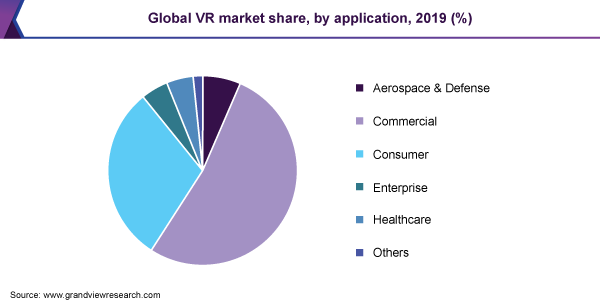
\includegraphics[width=\textwidth]{market_markets}
\captionsource{Światowy podział rynku VR pod względem wykorzystania aplikacji na rok 2019}{\url{https://www.grandviewresearch.com/industry-analysis/virtual-reality-vr-market/}}
\label{fig:market_m}
\end{figure}
 Poniżej przedstawiono kilka obszarów biznesowych w których rozwiązania XR funkcjonują często od wielu lat a ich rozwój i usprawnianie ciągle trwa. Do tych obszarów należą obszary takie jak lotnictwo, przemysł, medycyna oraz rozwiązania komercyjne~\cite{firmy}~\cite{vr4bus}. Obszary te zostały wybrane ze względu na popularność rozwiązań prezentowanych na rynku. Podział ten przedstawia rysunek~\ref{fig:market_m}.
\section{Lotnictwo i przemysł}
\label{sec:lotnictwo}
 Symulatory lotów były używane w szkoleniach wojskowych od wielu lat, ze względu na koszta które wynikały z używania prawdziwych samolotów jak i również potencjalnych zniszczeń który mogły powstać w trakcie szkolenia, a także bezpieczeństwa które symulator zapewniał. Dzięki temu popełnione błędy nie skutkowały utratą życia pilota. Równie ważnych aspektem jest fakt że podczas korzystania z symulatora można przetestować pilota w sytuacji awaryjnej, w której to należy podejmować szybkie decyzje a moment nie uwagi skutkuje rozbiciem maszyny. Dzięki temu w prawdziwej walce piloci są pewniejsi siebie oraz podejmują lepsze decyzje. Pierwsze symulatory powstały na początku XX wieku i były wykonane z drewna. Z biegiem czasem i rozwoju technologii pod koniec tego samego wieku zastąpiły je symulatory bazujące na mechanicznych częściach dzięki którym możliwy był ruch kokpitu, a obraz był wyświetlany na ekranach o dużej rozdzielczości. Koszty takiej maszyny mogły nawet przekraczać miliony dolarów. W związku z tym nastanie ery hełmów dla wirtualnej rzeczywistości przyniosło wiele rozwiązań które szybko zostały zastosowane. Dzięki użyciu gogli wyświetlających obraz, zwiększył się realizm or imersja symulacji, wizja pilota jest odwzorowana z uwzględnieniem ostrości widzenia, przeciążeń a także zapewniona jest wybiórcza wizja $360^o$, czyli pokazywany jest jedynie obszar widoczny w polu widzenia pilota, jednak może on dowolnie obserwować otoczenie wokół niego~\cite{del}. Kolejną instytucją w której wykorzystuje się technologie VR do szkolenia pracowników jest NASA. Wykorzystywanie nowoczesnych technologii w tej agencji kosmicznej nie jest nowością. W tym przypadku NASA zaprezentowało swój nowy symulator przeznaczony dla astronautów wyruszających na międzynarodową stację kosmiczną. W tym celu została wykorzystana technologia MR, dzięki której oprócz wirtualnych przedmiotów widzianych przez kosmonautę, były one również umiejscowione w tym samym miejscu w świecie rzeczywistym. Taki rodzaj symulacji zapewniał wyższy poziom realizmu przy zachowaniu niskich kosztów. System ten wspiera współpracę wielu użytkowników jednocześnie dzięki czemu zadania które są wykonywana w symulacji mogą również uwzględniać współpracę pomiędzy członkami załogi~\cite{nasa1}. Innym rodzajem symulacji, bazującym na treningu personelu są szkolenia personelu lotniczego. Nie dotyczy to jednak jedynie pilotów maszyn. Symulację dla personelu podczas pożaru w samolocie stworzyła firma EpicVR, która poprzez praktykę pokazała że pomimo dokładnych szkoleń i procedur, personel pokładowy wciąż popełnia błędy. Praktyka w symulatorze, dzięki zastosowaniu gogli do wirtualnej rzeczywistości sprawiła że już po kilku treningach, niektóre osoby wykonywały bezbłędnie procedury. Oczywiście praktyka takich procedur jest wykonywana nawet bez dostępu do nowoczesnej technologii, jednak w tym celu wymagana jest fizyczna wersja symulatora które nie są powszechnie dostępne~\cite{epicvr}. Są to jedynie przykładowe rozwiązania z tej dziedziny, z racji tego że wielkość fizycznych symulatorów pociąga za sobą duże koszta, wiele firm decyduje się na rozwiązania wirtualne. Innym sposobem stosowania symulacji jest symulacja linii produkcyjnej zastosowanej w Fordzie. Firma ta wprowadziła rozwiązania z dziedziny wirtualnej rzeczywistości zmniejszając ryzyko urazów o $70\%$, dla ponad 50 000 pracowników. Według danych podanych przez firmę, na dwa-trzy lata przed rozpoczęciem pracy nad nowym modelem zespół specjalistów analizuje w środowisku wirtualnym rozmieszczenie komponentów linii produkcyjnej tak aby zoptymalizować użycie siły pracowników aby nie doszło do przemęczenia, które mogłoby być przyczyną wypadku w fabryce. Aby osiągnąć najlepsze rezultaty podczas zbierania danych i zapewnić wymaganą jakość, zespół ten przeprowadza ponad 900 wirtualnych zadań zanim zostanie one fizycznie zbudowana, a oprócz podstawowych komponentów wykorzystują również technologie takie jak śledzenie ruchów całego ciała a także druk 3D~\cite{ford1}.
 
 Łatwo jest zauważyć jak duży wpływ rękawice wirtualnej rzeczywistości mają wpływ w tym obszarze rynku. Jeżeli firma chce symulować świat rzeczywisty w celu jak najlepszego szkolenia swoich pracowników, zależy jej aby były do tego wykorzystywane realne narzędzia. Będąc pilotem samolotu czy pracując fizycznie wykorzystujemy do tego nasze dłonie, w związku z tym podczas wykorzystania ich w trakcie treningu, ludzie również nabierają pamięci mięśniowej co pozwala podnieść poziom szkolenia a także rezultatów które dzięki niemu można osiągnąć. Między innymi ze względu na te powody, agencje takie jak NASA inwestują w technologię rękawic kontrolerów, sprawiając że powszechne rozwiązania symulatorów które będą wykorzystywane między innymi lotnictwie stają się coraz powszechniejsze~\cite{manus}. 
 
 \section{Architektura i wizualizacje}
\label{sec:architektura}
	Architekci jak mało która grupa deweloperów potrafią wykorzystać możliwości oferowane przez świat wirtualny. Od dawna grafika 3D jest powszechnie wykorzystywana w celu wizualizacji projektów, dzięki czemu klient bądź członkowie zespołu mają wgląd w to jak projekt będzie wyglądać po ukończeniu - wizja ta jest motorem napędowym całego projektu. DigitalVr postanowiło więc wykorzystać ten fakt i przenieść prezentację modeli na nowy poziom. Dzięki wykorzystaniu gogli VR, odbiorca jest w stanie przenieść się do ukończonego budynku zaprojektowanego w świecie wirtualnym, przejść się po nim, zmienić kolory ścian, obejrzeć je za dnia jak i nocy bądź poprzestawiać meble w pomieszczeniu. Jak twierdzą twórcy jest to swoiste przekazanie kluczy do drzwi wejściowych na lata przed powstaniem projektu w rzeczywistości. Twórcy wierzą że dzięki możliwością jakie zapewnia ich produkt, pewnego dnia ich rozwiązanie stanie się powszechnie używane. Obecnie rozwiązania takie nie tylko są oferowane przy użyciu gogli VR ale również aplikacji na smart-fony, które przy użyciu kamery telefonu pozwalają dopasowywać meble w pomieszczeniach domu bez opuszczania jego progu~\cite{arch}. Nie tylko architekci jednak wykorzystują wizualizację pomieszczeń w celu  przyciągnięcia klientów. Hotel Mariott International zamontował w niektórych swoich hotelach angielskie, czerwone budki telefoniczne w których można było skorzystać z zestawu Oculus Rift dzięki któremu klienci mogli przenieść się w wirtualną podróż do Londynu i na Hawaje~\cite{hotel2}. Współcześnie hotele takie jak Atlantis w Dubaju, Grand Oasis czy nawet powszechnie spotykany Holiday Inn oferują swoim klientom wirtualne wycieczki po hotelu zanim jeszcze zdecydują się na pobyt w ich posiadłości. Dzięki temu klienci wiedzą dokładnie na jakie atrakcje i standard mogą liczyć przy wyborze pokoju i lokacji~\cite{hotel1}. Wizualizacje przy wykorzystaniu XR nie służą jedynie przyciągnięciu klientów. Powszechnie stosuje się rozwiązania MR, AR oraz VR w celu optymalizacji pracy oraz redukcji błędów popełnianych przez pracowników.  Redukcja błędów jest szczególnie ważna w firmie Lockheed Martin, która wykorzystuje rozwiązania rozszerzonej rzeczywistości w celu budowania swoich samolotów wojskowych F-35. Wdrożenie tej technologii pozwoliło na zastąpienie grupy  wyszkolonych techników z latami doświadczenia, aplikacją która pokazuje pracowników jakie części muszę znaleźć się w danym elemencie. Brak zapamiętywania schematów a także aplikacja czuwająca nad pracą podczas składania poszczególnych elementów pozwoliła firmie usprawnić produkcję o $30\%$ a także uzyskać dokładność produkcyjną nawet do $96\%$. Podobną technikę wykorzystuje firma Boeing, która podczas montażu swoich samolotów wykorzystuje interaktywne instrukcje dzięki czemu w dowolnym momencie w łatwy sposób pracownicy mogą sprawdzić brakujące informacje. Jest to również zdecydowanie wygodniejsza forma niż manualne przeglądanie papierowych szkiców. Unikanie instrukcji papierowych jest stosowane nie tylko w przypadku  konstrukcji produktów lecz także podczas ich naprawy. Przykładem takiego zastosowania jest Panasonic Heating and Cooling Solutions - jest to dział ogrzewania i chłodzenia należący do firmy Pansonic. Dział ten wdrożył nowoczesne rozwiązanie dla swoich techników, pozwalając im przy wykorzystaniu  mieszanej rzeczywistości na konsultacje techników z centralą w celu rozwiązywania skomplikowanych problemów. Centrala po otrzymaniu obrazu jest w stanie na ekranie technika zaprezentować rozwiązanie danego problemu, znacznie skracając czas naprawy oraz redukując możliwość popełnienia błędów~\cite{pana}. Firma Ford natomiast oprócz zastosowania nowoczesnych technologii w swoich autach, stosuje ją również na etapie produkcji, i to nie tylko na linii produkcyjnej tak jak opisano to w sekcji~\ref{sec:lotnictwo}. Kolejnym przykładem nowoczesnego wykorzystania jest etap projektowania nowych aut. w tym celu projektancie mogą korzystać z gogli VR w celu wizualizacji swoich produktów w rzeczywistej skali jeszcze zanim zostaną one wyprodukowane, co pozwala na lepsze dopracowanie szczegółów każdego z aut~\cite{wiz1}. Firma Ford nie jest wyjątkiem w branży - rozwiązania XR oraz produkty rękawic kontrolerów stosowane są również w innych koncernach motoryzacyjnych takich jak BMW, Audi czy Toyota~\cite{manus}. Ostatnim rodzajem wizualizacji która zostanie opisana w tej sekcji jest klejne rozwiązanie stworzone przez agencję kosmiczną NASA. Tom Grubb który pracował nad tym narzędziem zauważył że badanie przestrzeni kosmicznej w szczególności związanej z liczbami dotyczącymi gwiazd w galaktyce, odbywało się poprzez używanie przestarzałych narzędzi opartych na pracy wielu baz danych. W związku z tym stworzył model w świecie wirtualnym który pozwalał na modelowanie tych danych w przystępnej dla ludzi formie czego rezultatem było osiągnięcie potwierdzenia wniosków z którymi do tej pory środowisko astronomów się nie zgadzało~\cite{nasa2}.
	
	 W tej sekcji przedstawiono kilka kolejnych rozwiązań dostępnych w firmach i agencjach które już teraz wykorzystują idealny kontroler - ludzką dłoń a także sposób stosowania nowych technologii w celu optymalizacji pracy a także przyciągnięcia nowych klientów. Jak widać w zależności od sektora a nawet działu,wizualizacje są wykorzystywane do najróżniejszych celów pozwalając na coraz to wydajniejszą pracę i lepsze efekty.
	
\section{Medycyna}
\label{sec:medycyna}
 Jednym z zastosowań obecnie używanych jest wspomniany już produkt Cynteract pomagający w fizjoterapii dłoni poprzez stawianie oporu a także interaktywny świat pozwalający zamienić trening w zabawę. Fizjoterapie nie jest jedynym obszarem w którym wykorzystuję się świat wirtualny. Jednym z bardzo imponujących zastosowań jest produkt o nazwie Snow World (z ang. Śnieżny świat), stworzony przez uniwersytet w Waszyngtonie. Produkt ten został stworzony aby pomagać pacjentom szpitala którzy doznali poważnych poparzeń ciała. Poprzez zastosowanie gogli VR zostają przeniesieni do śnieżnego świata w którym poprzez wizualizacje śniegu, bałwanów, pingwinów oraz innych typowych dla zimnego klimatu zwierząt i wydarzeń, pacjenci  mogą doświadczyć uczucia chłodu który jest generowany jedynie w naszej wyobraźni, jednak jak pokazują badania - mają bardzo realny efekt. Standardową procedurą jest podanie opioidów takich jak morfina, która redukuje ból w trakcie gojenia ran, jednak podczas oczyszczania ran czy zmian opatrunków skóra pacjentów poddawana jest dodatkowemu podrażnieniu co u niektórych pacjentów powoduje poważny ból pomimo zastosowania środków znieczulających, ponieważ pacjenci potrafią ponownie przeżywać doświadczenie poparzenia ich ciała. System wirtualnej rzeczywistości został zastosowany w celu dodatkowej redukcji bólu podczas tych bolesnych zabiegów poprzez przekierowanie skupienia pacjenta z bólu który przeżywa do wirtualnego środowiska. Zabieg przeprowadzono podczas  gdy pacjent grał w gry wideo na konsoli a także podczas przebywania w świecie VR. Rezultaty pokazały że samo przeniesienie skupienia na grę nie jest wystarczające - zastosowanie wirtualnego świata zmniejszyło odczucia bólu przez pacjenta o połowę~\cite{snow}. Tak jak w przypadku lotnictwa, również lekarze muszą trenować aby szczegółowo poznać procedury podczas wykonywania operacji. W tym obszarze wirtualne środowisko również przychodzi z pomocą. Oprócz pokazywania dobrze znanych zabiegów, w środowisku wirtualnym lekarze mogą ćwiczyć skomplikowane zabiegi, tak aby w trakcie prawdziwego zabiegu osiągnąć jak najlepsze rezultaty, tym samym ratując często ludzie życie. Symulacje zabiegów należą do grupy dość typowego wykorzystania wirtualnego świata, ponieważ praktycznie w każdym zawodzie można użyć tej technologii do polepszania umiejętności pracowników. Jednak w przypadku lekarzy, zastosowanie zaawansowanych i dokładnych rękawic sprawia że osoba ćwicząca dany zabieg nabiera pamięci mięśniowej a także uczy się obsługiwać dokładnie jak w rzeczywistości narzędzia które są wykorzystywane, często przy nietypowych zabiegach. Inną metodą wykorzystania XR jest tworzenie rozwiązań pomagających leczyć zespół stresu pourazowego poprzez stopniową ekspozycję pacjenta do bodźców i zastąpienie naturalnej reakcji pozytywnymi bodźcami. W podobny sposób tego rodzaju wizualizacje pozwalają pozbyć się różnego rodzaju lęków bądź nawet fobii takich jak lęk przed lataniem, wysokością, małymi pomieszczeniami czy wystąpieniami publicznymi. Wymienione zastosowania dobrze sprawdzają się w specjalistycznych placówkach, jednak istnieją również rozwiązania które dbają o ogólnie pojęte zdrowie człowieka poprzez naukę lepszego zarządzania stresem, relaksacji czy poprzez kurs medytacji - tego rodzaju rozwiązania mogą być wykorzystywane przez każdego z dostępem do gogli, sprawiając że ich użytek może być wyniesiony poza strefę rozrywkową~\cite{medycyna}.

\section{Rozrywka}
\label{sec:gry}
	Ostatnim działem opisanym w tej pracy jest jednocześnie strefa biznesu która rozpoczęła rozwój rynku wirtualnej rzeczywistości, dając jednocześnie początek innym technologiom a także pozwalając twórcą na wyobrażanie sobie coraz to nowych zastosowań w wielu dziedzinach biznesowych. Branża rozrywkowa poczynając od pierwszej maszyny Sensoramy aż do nowoczesnych gogli, napędza rynek konsumencki, sprawiając że technologia ta rośnie w popularności a także ludzie coraz częściej wiedzą jak z niej korzystać dzięki czemu łatwiej jest adoptowana w firmach. Mówiąc o rozrywce VR, najczęstszym skojarzeniem są gry komputerowe, które różnią się od bycia dokładnym odzwierciedleniem rzeczywistości do kompletnych abstrakcji. Oczywiście wszystkie opisane do tej pory zastosowania w biznesie, niejako mogą służyć jako przykłady dla gier. W ten sposób zostały stworzone symulatory lotów, które służą jedynie rozrywce, lecz często mogą być dobrym odwzorowaniem prawdziwego samolotu. W kontekście gier często użytkownik może sterować maszynami nie tylko powietrznymi ale także rożnego rodzaju pojazdami naziemnymi oraz wodnymi. Większość gier komputerowych które na chwilę obecną są wyświetlane na ekranie komputera, może zostać przeniesionych do VR, często z lepszymi doświadczeniami płynącymi z gry. Do najbardziej popularnych gier należą gry typu FPS (z ang. First Person Shooter), czyli gry polegające na strzelaniu i pokonywaniu przeciwników w których wcielamy się w postać i widzimy niejako jej oczami. Gracze mogą doświadczyć realnych wrażeń poprzez znalezienie się w środku pola bitwy, widoku i dzwięku eksplozji a także strzałów wokół nich. Do najpoważniejszych problemów tego typu gier należy możliwość poruszania się w świecie wirtualnym, tak aby był zachowany jak największy realizm. Kolejną pozycją która zajmuję dużą część rynku gier VR, są gry typu horror. Poprzez zastosowanie wizji $360^o$, wysokiej jakości grafiki, nastrojowego dźwięku oraz gwałtownych interakcji, gry te przenoszą użytkownika na wyższy poziom doznań, a w końcu to jest to czego fani tego typu gier oczekują. W przeciwieństwie do wymienionych do tej pory gatunków, wspomniane wcześniej symulatory nie cierpią z powodu problemu poruszania się, co sprawia że inercja użytkownika jest większa. Istnieją również gry strategiczne a także hazardowe które nie wymagają od użytkownika poruszania się, jednocześnie dostarczając lepszych doznań poprzez symulacje przebywania na polu bitwy na którym mamy widok "od środka" bądź też gdy użytkownik znajduję się w wirtualnym kasynie podczas gry w pokera~\cite{gry1}. Doświadczając rozrywki wirtualnego świata, należy wspomnieć o grze która przyczyniła się do rozgłosu technologii VR oraz jej popularyzacji jak żadna inna - Beat Saber to gra w której kontrolery zamieniają się w miecze w dwóch kolorach, którymi następnie należy niszczyć nadciągające w stronę użytkownika bloki. Bloki te mają kolory odpowiadające mieczom, i jedynie ten sam kolor miecza może je zniszczyć. Z pozoru bardzo prosta gra, jednak przyciągnęła ona wielu fanów a w szczególności pokazała przeciętnym graczom że może być tak ekscytująca jak gry 2D. Beat Saber sprzedała się w ilości ponad 100 000 egzemplarzy w przeciągu pierwszego miesiąca i została siódmą co do najlepiej ocenianych gier na platformie dla graczy Steam, pośród gier 2D jak i VR~\cite{gry2}. 
Oprócz zwykłych gier które służą czystej rozrywce, istnieje również zastosowanie gier w celach edukacyjnych. Gry takie wykorzystują stworzone środowisko w celu wizualizacji przedstawianego tematu w sposób bardziej intuicyjny niż samo opisywanie słowami, co wspomaga naukę u dzieci a nawet budzi większe zainteresowanie tematem. Do takich aplikacji należą na przykład aplikacje takie jak  Titans of Space, które prezentują układ słoneczny - do tej pory jedyną możliwością była prezentacja modeli które są wykonana w dużym pomniejszeniu. Innym przykładem jest aplikacja Anatomyou, która pozwala na podróż w głąb ludzkiego ciała. Rozwiązanie to sprawdza się w przypadku nauki biologii i anatomii. Istnieje wiele produktów które są przeznaczone do edukacji i szkoleń a rynek związany z grami wciąż rośnie~\cite{gry3}. Poniżej, na rysunku~\ref{fig:market_gry} pokazany jest podział rynku gier ze względu na wymagane komponenty. Rynek jest warty miliardy oraz wciąż rośnie co otwiera wiele możliwości zarówno dla twórców gier służących rozrywce jak i edukacji. Stwarza to możliwości zarówno dla nowych studiów produkcyjnych jak i dla biznesów zajmujących się wcielaniem w życie pomysłów dostarczonych przez inne osoby~\cite{gry1}.
   \begin{figure}[h]
\centering
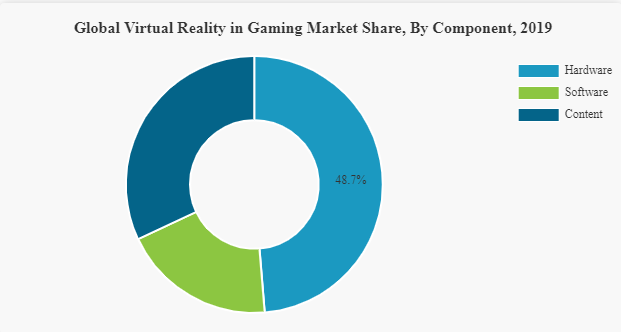
\includegraphics[width=\textwidth]{market_gry}
\captionsource{Światowy podział rynku gier VR pod względem komponentów na rok 2019}{\url{https://www.fortunebusinessinsights.com/industry-reports/virtual-reality-gaming-market-100271}}
\label{fig:market_gry}
\end{figure}